\documentclass[10pt]{article}
\usepackage{amsmath,amssymb}
\usepackage{xcolor}
\usepackage{graphicx}

% pdf hyperlinks
\definecolor{darkblue}{rgb}{0.0,0.0,0.3}

\usepackage[pdftex,
%                pagebackref=true,
		bookmarks,
		bookmarksopen=true,
		bookmarksnumbered=true,
		pdfauthor={Joseph Benzaken, Rasmus Tamstorf},
		pdftitle={Linear Shell Obstacle Course},
		colorlinks,
		linkcolor=darkblue,
		citecolor=darkblue,
		filecolor=black,
		urlcolor=darkblue,
		anchorcolor=darkblue,
		menucolor=black,
		breaklinks=true,
		pageanchor=true,
		plainpages=false,
		pdfpagelabels=true]{hyperref}

\newcommand{\Real}[0]{\mathbb{R}}

\setlength{\oddsidemargin}{-1in}
\addtolength{\oddsidemargin}{25mm} \setlength{\evensidemargin}{-1in}
\addtolength{\evensidemargin}{20mm} \setlength{\topmargin}{-1in}
\addtolength{\topmargin}{25mm} \setlength{\headheight}{0pt}
\setlength{\headsep}{0mm}
\setlength{\footskip}{10mm} \setlength{\textheight}{\paperheight}
\addtolength{\textheight}{-\footskip} \addtolength{\textheight}{-50mm}
\setlength{\textwidth}{\paperwidth} \addtolength{\textwidth}{-60mm}
\numberwithin{equation}{section}

\title{\normalfont The Linear Shell Obstacle Course}

\author{J. Benzaken, J. A. Evans, S. McCormick, R. Tamstorf}
\date{}

\begin{document}

\maketitle

\begin{figure}[h]
  \centering
  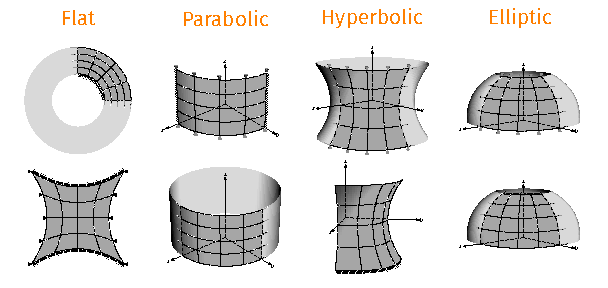
\includegraphics[width=\textwidth]{shells.pdf}
\end{figure}

\subsection*{Introduction}

Numerical validation for the linearized Kirchhoff-Love shell has often been performed by comparing the discrete displacement at a specified point in the geometry to a converged, high-resolution solution. Numerical observations throughout the shell community has led to a general consensus on what these values should be. However, in many cases, the computed and high-resolution approximations only agree up to a few digits of precision, and there is no underlying ``exactness'' with which they are associated. Furthermore, there are no theoretical error estimates in terms of these pointwise quantities because they are only equivalent to the available Sobolev estimates when the measured displacement field is sufficiently smooth. Finally, the ill-conditioning associated with the discrete linear system arising from discretization of the Kirchhoff-Love shell leads to numerical round-off errors, effectively rendering these ``high-resolution'' solutions unreliable for comparison.

The \textbf{\emph{linear shell obstacle course}} is intended to improve on these shortcomings and provide a validation tool for linearized Kirchhoff-Love shell codes. It addresses the issues by providing a suite of eight linear shell validation problems that are manufactured so that the exact solutions are known analytically. Together, these problems encompass all geometric configurations and boundary conditions that are admissible for the linearized Kirchhoff-Love shell. The linear shell obstacle course is embodied within a Mathematica notebook that contains the following:

\begin{itemize}
  \item The geometric parameterizations ${\bf x}$ for each problem.
  \item The displacement field ${\bf u}$ as a function of the convective coordinates $(\xi^1,\xi^2)$.
  \item The covariant membrane strain components $\alpha_{\alpha\beta}$ and the covariant bending strain components $\beta_{\alpha\beta}$ as a function of the convective coordinates $(\xi^1,\xi^2)$.
  \item The contravariant membrane stress components $A^{\alpha\beta}$ and the contravariant bending strain components $B^{\alpha\beta}$ as a function of the convective coordinates $(\xi^1,\xi^2)$, Young's modulus $E$, and Poisson's ratio $\nu$.
  \item The manufactured forcing function ${\bf f}$ in the Cartesian basis as a function of the convective coordinates $(\xi^1,\xi^2)$ that, when applied to the geometry, yields the above displacement, strain, and stress fields.
\end{itemize}

Together, these quantities are sufficient to compute the discretization error in both the displacement and the energy. The notebook can be viewed either in Mathematica or in the freely available \emph{Wolfram Player}\footnote{\url{https://www.wolfram.com/player/}}. The reason for providing the obstacle course in this format is to facilitate high-precision evaluation of the forcing functions, which is critical for obtaining reliable results (see additional discussion below).

The obstacle course is a result of the work published in \emph{``Nitsche’s Method for Variational Constrained Minimization Problems with Application to Membranes, Plates, and Shells'' by J. Benzaken, J. A. Evans, S. McCormick, and R. Tamstorf (submitted to CMAME)}. When using the linear shell obstacle course, please cite this paper.

\subsection*{Geometric Parameterizations}

The four basic geometric configurations of surfaces in $\Real^3$ are flat, parabolic, hyperbolic, and elliptic. To cover all of them, there are five parameterizations: two flat geometries and one of each of the other types of geometries. Each of the non-flat geometries are used twice with different boundary conditions, leading to a total of eight problems. All geometries are parameterized using biquadratic B-splines or a single NURBS patch. Moreover, each parameterization is over one isogeometric element and, hence, contains nine degrees of freedom. Obtaining equivalent parameterizations of a higher polynomial degree and/or finer mesh resolution requires degree elevation and/or knot insertion routines, respectively.

\subsection*{Boundary Conditions}

The linearized Kirchhoff-Love shell accommodates four types of boundary conditions: clamped, simply supported, symmetric, and free. A simply supported shell is one where the boundary displacement is zero while the normal rotation is unconstrained. A shell with symmetric boundary conditions is one where the boundary displacement is unconstrained while the normal rotation is zero. A shell with free boundary conditions is one where both the boundary displacement and the normal rotation are unconstrained. From energetic principles, this implies that the quantities energetically conjugate to those that are unconstrained must vanish. For simply supported structures, this is the bending moment; for those with symmetric boundaries, this is the ersatz traction; and for those with free boundaries, this is both. Since it is nearly impossible to manufacture a solution exhibiting exactly these properties, our linear shell obstacle course simply emulates this behavior by instead prescribing inhomogeneous Dirichlet boundary conditions in lieu of those that should be unconstrained. These four boundary condition types are combined with the aforementioned four geometry classes to obtain the complete set of eight problems in our linear shell obstacle course.

\subsection*{Displacement Fields}

As described in the previous section, the prescribed displacement fields are used to effectively emulate the boundary conditions that can be encountered during the simulation of the linearized Kirchhoff-Love shell. For example, geometries with clamped boundaries have zero displacement and zero normal rotation along that boundary while those that are simply supported have zero displacement with nonzero rotation along the boundary. Many of the displacement fields are constructed so that they align with the convective coordinates or are orthogonal to the shell midsurface. To accommodate this, we frequently express the displacement fields in terms of the in-plane covariant basis vector fields ${\bf a}_1$ and ${\bf a}_2$ and/or the midsurface normal director ${\bf a}_3$ that are constructed through derivatives of the geometric mapping. Note that the geometric parameterizations for all problems are such that $\xi^1,\xi^2 \in [0,1]$ and, hence, the same holds for all of the displacement fields, stress and strain tensors, and forcing functions.

\subsection*{Obstacle Course}

Combining the above set of geometries, boundary conditions, and displacement fields leads to the following list of eight problems that comprise the linear shell obstacle course:
\begin{enumerate}
  \item[] \underline{Flat Geometries}
  \begin{itemize}
    \item \textbf{\emph{Quarter Annulus}}: a NURBS-mapped domain with symmetry along the radial edges of the domain, clamped on the inner radius, and free on the outer radius.
      \begin{equation*}
        {\bf u}\left( \xi^1, \xi^2 \right) = \left( \frac{\xi^1}{\|{\bf a}_1\|} \right) {\bf a}_1 + \left( e^{\xi^1} - 1 \right)\xi^1 {\bf a}_3
      \end{equation*}
    \item \textbf{\emph{Astroid}}\footnote{Technically, it is not truly an astroid but only an astroid-like domain}: a B-spline-mapped domain with two opposite clamped edges and two opposite simply supported edges.
    \begin{equation*}
      {\bf u} \left( \xi^1, \xi^2 \right) := \left( \begin{array}{c}
      u_x\\
      u_y\\
      u_z \end{array} \right) = \left( \begin{array}{c}
        \left( \xi^1 - 1 \right)^2 \left( \xi^1 \right)^2 \left( \frac{1}{2} - \xi^2 \right) (1 - \xi^2) \xi^2 \vspace{1pt}\\
        \left( \xi^2 - 1 \right)^2 \left( \xi^2 \right)^2 \left( \frac{1}{2} - \xi^1 \right) (1 - \xi^1) \xi^1 \vspace{1pt}\\
        \left( 1 - \xi^1 \right) \xi^1 \sin(\pi \xi^1) \sin(\pi \xi^2) \end{array} \right)
    \end{equation*}
  \end{itemize}
  \item[] \underline{Parabolic Geometries}
  \begin{itemize}
    \item \textbf{\emph{Quarter Cylinder}}: a NURBS-mapped domain with two opposite clamped edges and two opposite simply supported edges.
    \begin{equation*}
      {\bf u}\left( \xi^1, \xi^2 \right) := - \left( \xi^1 - 1\right)^2 \left( \xi^1 \right)^2 \xi^2 \left(\xi^2 - 1 \right) {\bf a}_3
    \end{equation*}
    \item \textbf{\emph{Full Cylinder}}: a NURBS-mapped domain with symmetry along the radial edges of the domain and free on the other edges.
    \begin{equation*}
      {\bf u}\left( \xi^1, \xi^2 \right) := \frac{1}{2} \cos \left( \pi \xi^1 \right) {\bf a}_3
    \end{equation*}
  \end{itemize}
  \item[] \underline{Hyperbolic Geometries}
  \begin{itemize}
    \item \textbf{\emph{Inflated Hyperbolic Paraboloid}}: a B-spline-mapped domain with two opposite simply supported edges and two symmetric edges.
    \begin{equation*}
      {\bf u}\left( \xi^1, \xi^2 \right) := \left( \begin{array}{c}
      u_x\\
      u_y\\
      u_z \end{array} \right) = \left( \begin{array}{c}
        \sqrt{2} \left( \left( \xi^1 \right)^2 - 1 \right) \left( \xi^2 -1 \right) \xi^2 \vspace{1pt}\\
        \sqrt{2} \left( \xi^1 - 2 \right) \xi^1 \left( \xi^2 -1 \right) \xi^2 \vspace{1pt}\\
        0 \end{array} \right)
    \end{equation*}
    \item \textbf{\emph{Hyperbolic Paraboloid Diving Board}}: a B-spline-mapped domain with one clamped edge and the remaining three edges being free.
    \begin{equation*}
      {\bf u}\left( \xi^1, \xi^2 \right) := \left( \begin{array}{c}
      u_x\\
      u_y\\
      u_z \end{array} \right) = \left( \begin{array}{c}
        \xi^2 \sin \left( \frac{\pi}{2} \xi^2 \right) \vspace{1pt}\\
        \xi^2 \sin \left( \frac{\pi}{2} \xi^2 \right) \vspace{1pt}\\
        0 \end{array} \right)
    \end{equation*}
  \end{itemize}
  \item[] \underline{Elliptic Geometries}
  \begin{itemize}
    \item \textbf{\emph{Inflated Hemisphere}}: a B-spline-mapped domain with two opposite simply supported edges and two symmetric edges.
    \begin{equation*}
      {\bf u}\left( \xi^1, \xi^2 \right) := - \sin \left( \pi \xi^1 \right) {\bf a}_3
    \end{equation*}
    \item \textbf{\emph{Stretched Hemisphere}}: a B-spline-mapped domain with two symmetric edges, a clamped hole along the top, and free equator.
    \begin{equation*}
      {\bf u}\left( \xi^1, \xi^2 \right) := \left( \begin{array}{c}
      u_x\\
      u_y\\
      u_z \end{array} \right) = \left( \begin{array}{c}
        0 \vspace{1pt}\\
        0 \vspace{1pt}\\
        \left( \xi^1 - 1 \right)\left( e - e^{\xi^1} \right) \end{array} \right)
    \end{equation*}
  \end{itemize}
\end{enumerate}

The hyperbolic and elliptic geometries are not true hyperbolic paraboloids and hemispheres because this would require a rational mapping. However, they are approximations thereof obtained by setting the NURBS weights to unity in otherwise exact hyperbolic and elliptic mappings. This approximation does not alter the classification of these geometries as hyperbolic and elliptic. The choice not to use the exact mapping is made for computational ease because the associated forcing functions for true, rational mappings become unwieldy quickly.

All of the above functions are readily available for computation in the Mathematica notebook. In addition, there are plots of the resulting displaced geometries for visual reference. For further details, refer to the obstacle course notebook.

\subsection*{Forcing Functions}

The forcing functions necessary to produce the prescribed displacement field can be manufactured by applying the differential operators arising from the strong formulation of the linearized Kirchhoff-Love shell to the displacement fields. These differential operators are defined over the shell manifold and are up to and including fourth order. The resulting expressions therefore become quite complex rather quickly, but they are all contained within the notebook.

\subsection*{Strain and Stress Components}

Given a geometry, a set of boundary conditions, and a forcing function, the displacement field can be computed by solving the Kirchhoff-Love shell equations. The result should be compared to the displacement field given above for each of the problems. The difference between the two is usually measured in either the $L^2$ norm or in the energy norm. To compute the latter, we provide the contravariant components of the stress tensors and the covariant components of the strain tensors for each of the problems. Both the stress tensors and the strain tensors are decomposed into membrane contributions and bending contributions to allow the solution to be evaluated for different shell thicknesses.

The covariant membrane and bending strain components are denoted $\alpha_{\alpha\beta}$ and $\beta_{\alpha\beta}$, respectively, while the contravariant membrane and bending stress components are denoted $A^{\alpha\beta}$ and $B^{\alpha\beta}$, respectively. The stress tensors are provided for convenience since they can simply be obtained from the strain tensors using the linear constitutive law. In particular, $A^{\alpha\beta} = \zeta \mathbb{C}^{\alpha\beta\lambda\mu} \alpha_{\lambda\mu}$ and $B^{\alpha\beta} = \frac{\zeta^3}{12} \mathbb{C}^{\alpha\beta\lambda\mu} \beta_{\lambda\mu}$, where $\zeta$ is the shell thickness. Additionally, the constitutive model is given by
\begin{equation*}
 \mathbb{C}^{\alpha\beta\lambda\mu} = \frac{E}{2(1+\nu)}\left( a^{\alpha\lambda}a^{\beta\mu} + a^{\alpha\mu}a^{\beta\lambda} + \frac{2\nu}{1-\nu}a^{\alpha\beta}a^{\lambda\mu} \right)
 \end{equation*}
 where $E$ is Young's modulus, $0 \le \nu \le \frac{1}{2}$ is Poisson's ratio, and $a^{\alpha\beta}$ are the contravariant metric coefficients.


\subsection*{Expression Evaluations}

The strain and stress components, as well as the forcing functions, become unwieldy rather quickly due to the complexity associated with differential operators defined over manifolds. As such, for many of the problems, it is ill-advised and perhaps even impossible to use these functions directly in standard finite element codes because in some cases, evaluating these functions is numerically unstable. In those cases, severely deteriorated or no convergence will be observed.

To remedy this, it is recommended that the forcing function be evaluated at the quadrature points in high precision, and the results be truncated thereafter to the working precision. These values should then be saved to a location where they can later be read by the finite element code. Inside of the code, instead of calling on the forcing function to be evaluated at the quadrature points, these files are read and used for computing the $L^2$-projection of the forcing function on to the test space of finite element basis functions. Due to the severely nonlinear nature of these functions, it is also recommended that these functions be over-integrated with a numerical quadrature rule of a much higher precision than what is typically required for the chosen discretization. Finally, it is recommended that a similar approach be used in computation of the strain energy error because, once again, the corresponding strains and stresses are very nonlinear and numerically unstable in some instances.

\end{document}
